\section{Introduction}


\section{Related Work}



\section{The Model}

Let $R = \{r_1, r_2, \ldots, r_N\}$ is a set of all possible N requirements for software or company and each requirement $r_i \in R$ has its cost and profit, $cost_i \in \mathbb{Z}^+$ and $profit_i \in \mathbb{Z}^+$, to be performed. The cost is whatever company have to pay to resolve requirements, for example, money, time and etc. The profit is whatever company get by resolving requirements, for example, user satisfaction. In this project, we assumed that all requirements are independent. It means, there is no prerequisite of requirements. The cost vector $Cost$ and the profit vector $Profit$ for requirements are denoted by 
\[
Cost = \{cost_1, cost_2, \ldots, cost_N\}
\]
\[
Profit = \{profit_1, profit_2, \ldots, profit_N\}
\]

The company always wants to select requirements for the next release to get the highest sum of profits in the limited budget. Let the decision vector $x = \{x_1, x_2, \ldots, x_n\} \in \{0, 1\}$ where $x_i$ is 1 if requirement $i$ is selected and 0 otherwise. Then our objective function can be written as below:
\[
maximize \sum_{i = 1}^{N} profit_i \cdot x_i
\]
subject to
\[
\sum_{i = 1}^{N} cost_i \cdot x_i \leq B
\]
for some bound $B \in \mathbb{Z}^+$ which represents the limited budget.




\section{Algorithms}
\subsection{Analytic Hierarchy Process(AHP)}
\subsection{Integer Linear Programming(ILP)}
Integer Linear Programming(ILP) is optimization method whose objective function and constraints are linear, and all variables are integer. We referred ILP at the paper \textit{<An Integer Linear Programming approach to the single and bi-objective Next Release Problem>} by N Veerapen et al. This paper used ILP solver named \textit{CPLEX}, but it is commercial solver so we used \textit{PuLP}(modeler) and \textit{Gurobi}(solver) for this project. \textit{PuLP} is free open source software so users can use it by pip install. However general \textit{Gurobi} solver is commercial one so we registered to \textit{Gurobi (www.gurobi.com)} and used \textit{Gurobi} academic version. \\
\subsection{Simulated Annealing(SA)}
\subsection{Genetic Algorithm(GA)}
\subsection{NSGA-II}

\begin{table*}
  \caption{Profit Comparison}
  \label{tab:commands}
  \begin{tabular}{cccccl}
    \toprule
    &eclipse-log&firefox-log&firefox-priority&firefox-comments+priority\\
    \midrule
    Real Cost&50699.70190&262945.49581&262945.49581&262945.49581 \\
    Real Profit&3489.63592&13025.88085&12210&26332.88085 \\
    \hline
    SA&3702.85182&13524.93411&16300.0&28358.2295685 \\
    GA&3793.5045&13662.38600&16303.0&28522.11861 \\
    NSGA-II&3822.47741&13700.52067&16518.33333&28729.33476 \\
    ILP&3825.42768&13768.44722&16336.0&28845.23124 \\
    AHP&3810.3125825&13758.5577962&16249.0&28811.2749907 \\
    \bottomrule
  \end{tabular}
\end{table*}
% end the environment with {table*}, NOTE not {table}!

\begin{figure*}[h]
\begin{subfigure}{\columnwidth}
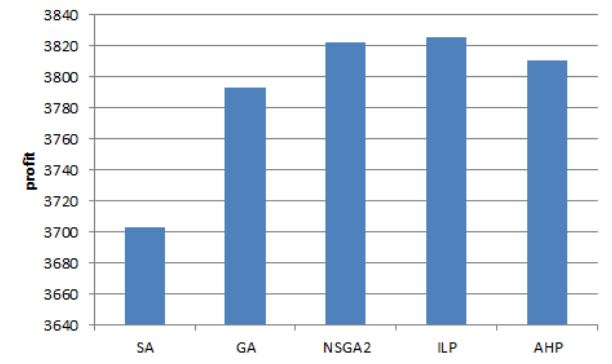
\includegraphics[width=0.9\linewidth]{bugzilla_eclipse_log(comments)_2016meancost.JPG}
\caption{bugzilla-eclipse-log(comments)-2016meancost}
\label{fig:subim1}
\end{subfigure}
\begin{subfigure}{\columnwidth}
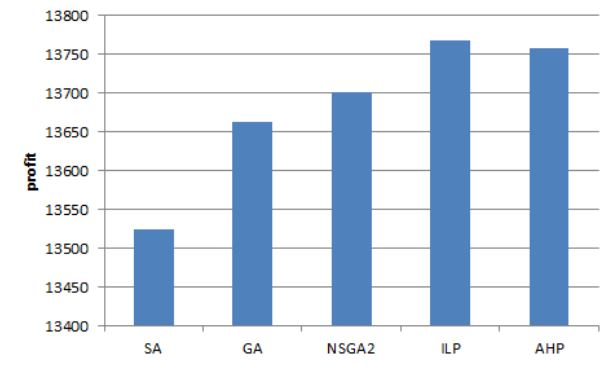
\includegraphics[width=0.9\linewidth]{bugzilla_firefox_log(comments)_2016meancost.JPG}
\caption{bugzilla-firefox-log(comments)-2016meancost}
\label{fig:subim2}
\end{subfigure}
\begin{subfigure}{\columnwidth}
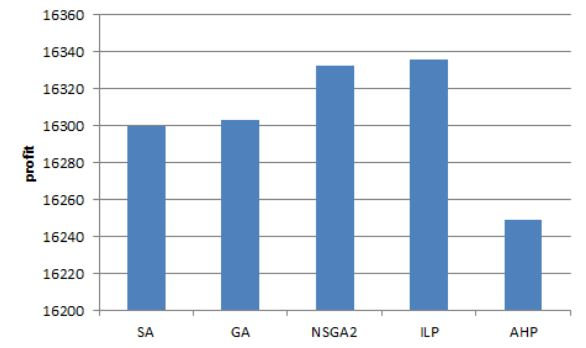
\includegraphics[width=0.9\linewidth]{bugzilla_firefox_priority_2016meancost.JPG}
\caption{bugzilla-firefox-priority-2016meancost}
\label{fig:subim3}
\end{subfigure}
\begin{subfigure}{\columnwidth}
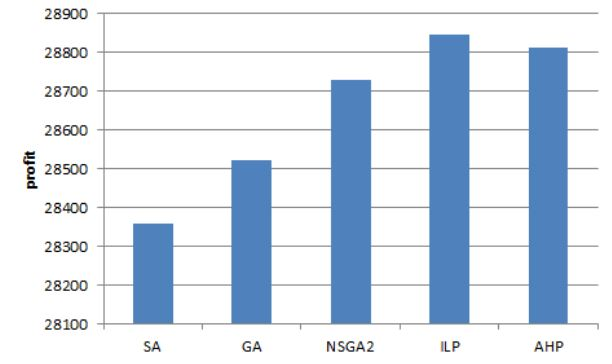
\includegraphics[width=0.9\linewidth]{bugzilla_firefox_comments-priority_2016meancost.JPG}
\caption{bugzilla-firefox-comments+priority-2016meancost}
\label{fig:subim4}
\end{subfigure}

\caption{Profit Comparison for each dataset}
\label{fig:image1}
\end{figure*}

\begin{figure*}[h]
\begin{subfigure}{\columnwidth}
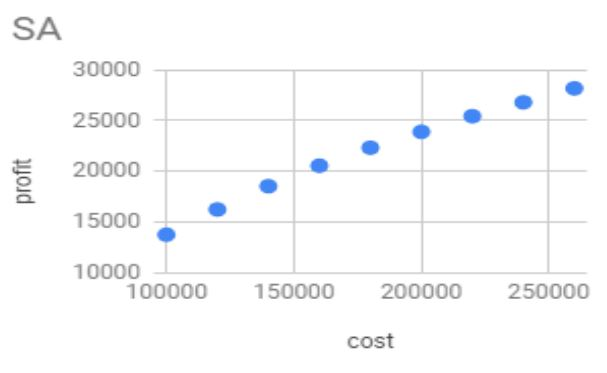
\includegraphics[width=0.9\linewidth]{SA-correlation.JPG}
\caption{SA}
\label{fig:subim5}
\end{subfigure}
\begin{subfigure}{\columnwidth}
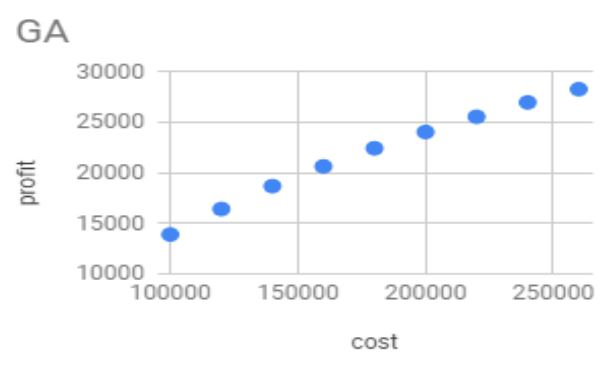
\includegraphics[width=0.9\linewidth]{GA-correlation.JPG}
\caption{GA}
\label{fig:subim6}
\end{subfigure}
\begin{subfigure}{\columnwidth}
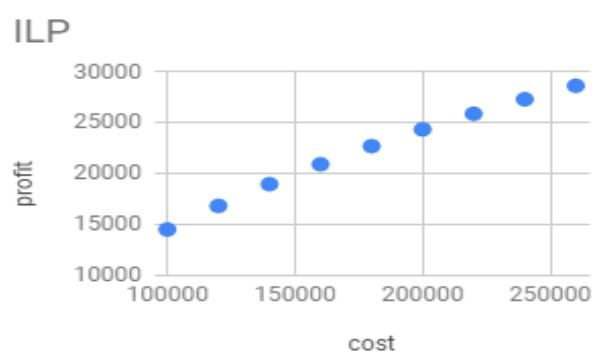
\includegraphics[width=0.9\linewidth]{ILP-correlation.JPG}
\caption{ILP}
\label{fig:subim7}
\end{subfigure}
\begin{subfigure}{\columnwidth}
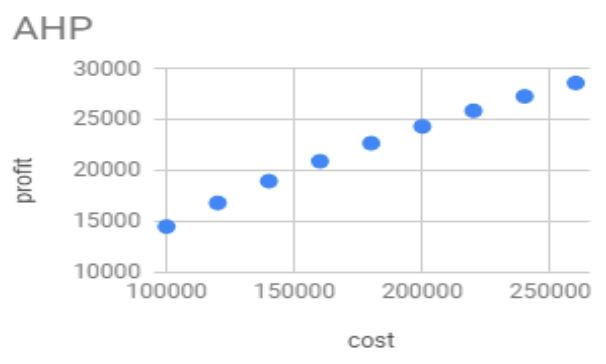
\includegraphics[width=0.9\linewidth]{AHP-correlation.JPG}
\caption{AHP}
\label{fig:subim8}
\end{subfigure}

\caption{Cost-Profit Correlation}
\label{fig:image2}
\end{figure*}

\begin{figure*}[h]
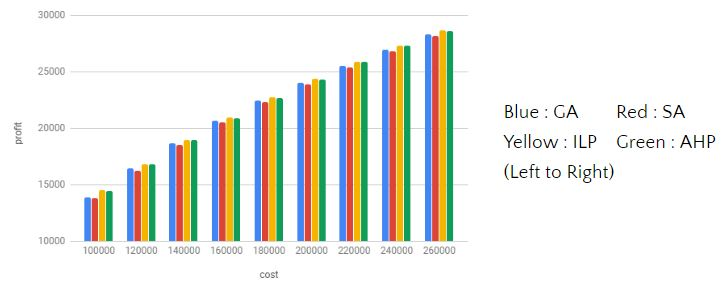
\includegraphics[width=0.9\linewidth]{cost-profit-together.JPG}
\caption{Cost-Profit Correlation in one graph}
\label{fig:image3}
\end{figure*}

\section{result}
At first experiment, we applied five algorithms to four datasets and compared the maximum profit each other. In \textbf{table 1}, upper two rows are real cost sum and real profit sum of each datasets. Below these rows, there are maximum profits for each algorithms in four datasets. At the result, every maximum profits are bigger than real profit sum. Also, consumed time to return maximum profit was exceedingly short in ILP and AHP, rather than SA, GA, and NSGA-II. \\
\textbf{Figure 1} is the graphs of \textbf{table 1}. Each graph expresses the maximum profit of five algorithms. At the result, the maximum profit of ILP is the biggest, and the maximum profit of NSGA-II and AHP is bigger than the maximum profit of SA and GA in most case. Except ILP and AHP, maximum profit is high in order of NSGA-II, GA, then SA. Peculiar thing is that, in dataset \textit{bugzilla-firefox-priority-2016meancost}, NSGA-II is largely bigger than other four algorithms. The reason we suppose is that other three datasets' profit is variety because the number of comments is not bounded, but this dataset's profit is priority, which is varied only in 1, 2, 3, 4, and 5 points. In this case, requirements can be seen more similar each other than other datasets. This difference could influence the difference of the result.\\
At experiment 2, we applied four algorithms except NSGA-II to dataset \textit{bugzilla-firefox-comments+priority-2016meancost}. At this experiment, we got the maximum profits while changing the cost constraints. The result is expressed in \textbf{Figure 2} and \textbf{Figure 3}. \textbf{Figure 2} expresses maximum profits on each cost, and \textbf{Figure 3} is integrating graph of \textbf{Figure 2} because of comparing the difference for four algorithms. \\
The result is that they are all increasing almost linearly and similarly. One of the reasons to perform this experiment was that we wondered if there is a peculiar part in cost-profit graph.(if there is exceeding increase in profit) And at the result, there is no prominently peculiar part, and all the results are increasing normally.
\subsection{Type Changes and {\itshape Special} Characters}


\subsection{Math Equations}
You may want to display math equations in three distinct styles:
inline, numbered or non-numbered display.  Each of
the three are discussed in the next sections.

\subsubsection{Inline (In-text) Equations}
A formula that appears in the running text is called an
inline or in-text formula.  It is produced by the
\textbf{math} environment, which can be
invoked with the usual \texttt{{\char'134}begin\,\ldots{\char'134}end}
construction or with the short form \texttt{\$\,\ldots\$}. You

few examples of in-text equations in context. Notice how
this equation:
\begin{math}
  \lim_{n\rightarrow \infty}x=0
\end{math},
set here in in-line math style, looks slightly different when
set in display style.  (See next section).

\subsubsection{Display Equations}
A numbered display equation---one set off by vertical space from the
text and centered horizontally---is produced by the \textbf{equation}
environment. An unnumbered display equation is produced by the
\textbf{displaymath} environment.

Again, in either environment, you can use any of the symbols
and structures available in \LaTeX\@; this section will just
give a couple of examples of display equations in context.
First, consider the equation, shown as an inline equation above:
\begin{equation}
  \lim_{n\rightarrow \infty}x=0
\end{equation}
Notice how it is formatted somewhat differently in
the \textbf{displaymath}
environment.  Now, we'll enter an unnumbered equation:
\begin{displaymath}
  \sum_{i=0}^{\infty} x + 1
\end{displaymath}
and follow it with another numbered equation:
\begin{equation}
  \sum_{i=0}^{\infty}x_i=\int_{0}^{\pi+2} f
\end{equation}
just to demonstrate \LaTeX's able handling of numbering.

\subsection{Citations}



\subsection{Tables}
Because tables cannot be split across pages, the best
placement for them is typically the top of the page
nearest their initial cite.  To
ensure this proper ``floating'' placement of tables, use the
environment \textbf{table} to enclose the table's contents and
the table caption.  The contents of the table itself must go
in the \textbf{tabular} environment, to
be aligned properly in rows and columns, with the desired
horizontal and vertical rules.  Again, detailed instructions
on \textbf{tabular} material
are found in the \textit{\LaTeX\ User's Guide}.

Immediately following this sentence is the point at which
Table is included in the input file; compare the
placement of the table here with the table in the printed
output of this document.


To set a wider table, which takes up the whole width of the page's
live area, use the environment \textbf{table*} to enclose the table's
contents and the table caption.  As with a single-column table, this
wide table will ``float'' to a location deemed more desirable.
Immediately following this sentence is the point at which
Table is included in the input file; again, it is
instructive to compare the placement of the table here with the table
in the printed output of this document.




It is strongly recommended to use the package booktabs
and follow its main principles of typography with respect to tables:
\begin{enumerate}
\item Never, ever use vertical rules.
\item Never use double rules.
\end{enumerate}
It is also a good idea not to overuse horizontal rules.


\subsection{Figures}



As was the case with tables, you may want a figure that spans two
columns.  To do this, and still to ensure proper ``floating''
placement of tables, use the environment \textbf{figure*} to enclose
the figure and its caption.  And don't forget to end the environment
with \textbf{figure*}, not \textbf{figure}!


\subsection{Theorem-like Constructs}

Other common constructs that may occur in your article are the forms
for logical constructs like theorems, axioms, corollaries and proofs.
ACM uses two types of these constructs:  theorem-like and
definition-like.

Here is a theorem:
\begin{theorem}
  Let $f$ be continuous on $[a,b]$.  If $G$ is
  an antiderivative for $f$ on $[a,b]$, then
  \begin{displaymath}
    \int^b_af(t)\,dt = G(b) - G(a).
  \end{displaymath}
\end{theorem}

Here is a definition:
\begin{definition}
  If $z$ is irrational, then by $e^z$ we mean the
  unique number that has
  logarithm $z$:
  \begin{displaymath}
    \log e^z = z.
  \end{displaymath}
\end{definition}

The pre-defined theorem-like constructs are \textbf{theorem},
\textbf{conjecture}, \textbf{proposition}, \textbf{lemma} and
\textbf{corollary}.  The pre-defined de\-fi\-ni\-ti\-on-like constructs are
\textbf{example} and \textbf{definition}.  You can add your own
constructs using the \textsl{amsthm} interface.  The
styles used in the \verb|\theoremstyle| command are \textbf{acmplain}
and \textbf{acmdefinition}.

Another construct is \textbf{proof}, for example,

\begin{proof}
  Suppose on the contrary there exists a real number $L$ such that
  \begin{displaymath}
    \lim_{x\rightarrow\infty} \frac{f(x)}{g(x)} = L.
  \end{displaymath}
  Then
  \begin{displaymath}
    l=\lim_{x\rightarrow c} f(x)
    = \lim_{x\rightarrow c}
    \left[ g{x} \cdot \frac{f(x)}{g(x)} \right ]
    = \lim_{x\rightarrow c} g(x) \cdot \lim_{x\rightarrow c}
    \frac{f(x)}{g(x)} = 0\cdot L = 0,
  \end{displaymath}
  which contradicts our assumption that $l\neq 0$.
\end{proof}

\section{Conclusions}
This paragraph will end the body of this sample document.
Remember that you might still have Acknowledgments or
Appendices; brief samples of these
follow.  There is still the Bibliography to deal with; and
we will make a disclaimer about that here: with the exception
of the reference to the \LaTeX\ book, the citations in
this paper are to articles which have nothing to
do with the present subject and are used as
examples only.
%\end{document}  % This is where a 'short' article might terminate



\appendix
%Appendix A
\section{Headings in Appendices}
The rules about hierarchical headings discussed above for
the body of the article are different in the appendices.
In the \textbf{appendix} environment, the command
\textbf{section} is used to
indicate the start of each Appendix, with alphabetic order
designation (i.e., the first is A, the second B, etc.) and
a title (if you include one).  So, if you need
hierarchical structure
\textit{within} an Appendix, start with \textbf{subsection} as the
highest level. Here is an outline of the body of this
document in Appendix-appropriate form:
\subsection{Introduction}
\subsection{The Body of the Paper}
\subsubsection{Type Changes and  Special Characters}
\subsubsection{Math Equations}
\paragraph{Inline (In-text) Equations}
\paragraph{Display Equations}
\subsubsection{Citations}
\subsubsection{Tables}
\subsubsection{Figures}
\subsubsection{Theorem-like Constructs}
\subsubsection*{A Caveat for the \TeX\ Expert}
\subsection{Conclusions}
\subsection{References}
Generated by bibtex from your \texttt{.bib} file.  Run latex,
then bibtex, then latex twice (to resolve references)
to create the \texttt{.bbl} file.  Insert that \texttt{.bbl}
file into the \texttt{.tex} source file and comment out
the command \texttt{{\char'134}thebibliography}.
% This next section command marks the start of
% Appendix B, and does not continue the present hierarchy
\section{More Help for the Hardy}

Of course, reading the source code is always useful.  The file
\path{acmart.pdf} contains both the user guide and the commented
code.

\begin{acks}
  The authors would like to thank Dr. Yuhua Li for providing the
  MATLAB code of the \textit{BEPS} method.

  The authors would also like to thank the anonymous referees for
  their valuable comments and helpful suggestions. The work is
  supported by the \grantsponsor{GS501100001809}{National Natural
    Science Foundation of
    China}{http://dx.doi.org/10.13039/501100001809} under Grant
  No.:~\grantnum{GS501100001809}{61273304}
  and~\grantnum[http://www.nnsf.cn/youngscientists]{GS501100001809}{Young
    Scientists' Support Program}.

\end{acks}
